% !TeX root = ../cyh.tex

\chapter{ArceOS 内核}

\section{ArceOS 概述}

ArceOS 是一个基于 Rust 语言开发的组件化操作系统,它是目标宏内核 starry-next 的基底,为宏内核提供了底层组件和相应接口的支持。ArceOS 由以下模块组成:

\begin{itemize}
\item axruntime:负责从裸机环境启动并进行初始化工作,在进入应用程序的main函数之前完成一系列准备操作,如日志初始化、内存分配器初始化、平台设备初始化等。
\item axhal:硬件抽象层,负责指定平台的启动和初始化过程,通过针对不同的硬件平台和架构实现特定的代码,将底层硬件的差异封装起来,为上层提供统一的接口。支持多种架构,如 x86\_64、riscv64、aarch64、loongarch64。
\item axconfig:存储平台特定的常量和参数,如物理内存基地址、内核加载地址、栈大小等。
\item axlog:提供多级格式化日志记录功能。
\item axalloc:全局内存分配器,实现了一套内存分配和管理算法,负责为系统和应用程序分配内存。在需要内存时,会根据请求的大小和内存状态,从空闲内存池中分配合适的内存块,并记录内存的使用情况。
\item axdisplay:图形模块,用于处理图形相关的操作。
\item axfs:文件系统模块,实现了文件系统的基本操作,如文件的创建、读取、写入、删除等。会维护文件系统的元数据(如文件的目录结构、文件属性等),并将文件数据存储在存储设备上。
\item axnet:网络模块,封装了底层网络栈的功能,提供了类似 POSIX 的网络 API。在接收到网络请求时,会将请求传递给底层网络栈进行处理,并将处理结果返回给上层应用程序。
\item axdriver:设备驱动模块,负责检测和初始化各种设备驱动,并将检测到的设备封装到 AllDevices 结构体中供上层子系统使用。
\item axtask:任务管理模块,负责维护一个任务队列,提供任务创建、调度、睡眠、终止等接口。调度算法会根据任务的优先级、状态等因素,决定哪个任务应该在何时运行。在任务调度时,会保存当前任务的上下文信息,加载下一个任务的上下文信息,实现任务的切换。
\item axsync:同步原语模块,通过硬件提供的原子操作或软件算法实现同步原语。例如,互斥锁可以使用原子操作来实现对共享资源的互斥访问,确保同一时间只有一个任务可以访问共享资源。
\item axdma:DMA 模块,用于管理直接内存访问(DMA)操作,允许某些硬件子系统在不经过 CPU 控制的情况下直接访问系统内存。
\item axmm:虚拟内存管理模块,其主要功能在于对虚拟内存进行高效的分配、映射以及管理,确保系统和应用程序能够合理、安全地使用内存资源。
\item axns:命名空间模块,用于控制线程间系统资源共享。它通过命名空间来管理系统资源,包括虚拟地址空间、工作目录和文件描述符,用于在不同场景下访问系统资源。
\end{itemize}

\begin{figure}
  \centering
  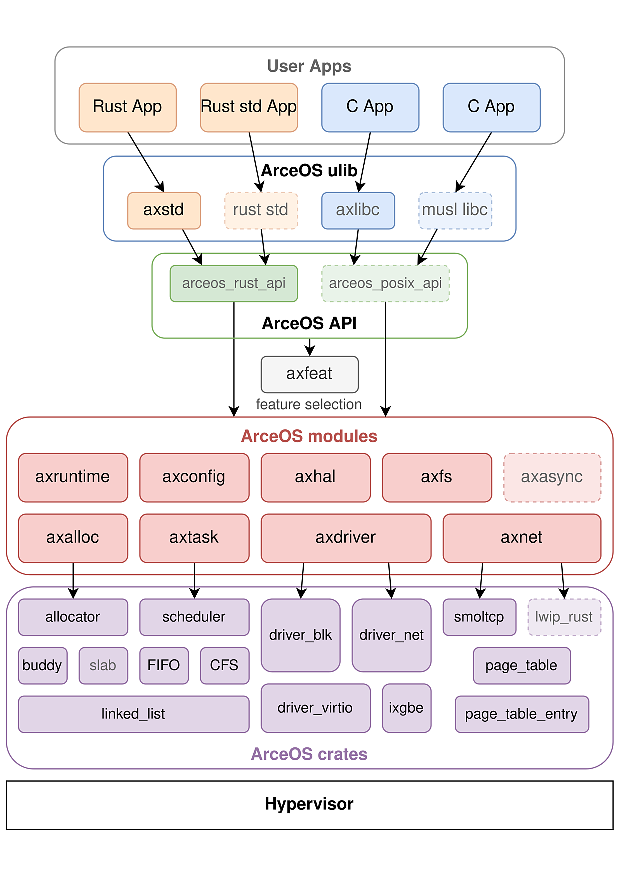
\includegraphics[width=0.5\linewidth]{ArceOS (1).pdf}
  \caption{ArceOS 内核结构图}
  \label{fig:ArceOS}
\end{figure}

每个模块包含多个组件,不同模块组合组合为应用程序提供底层支持。其中应用运行时模块
(axruntime)、硬件抽象层模块(axhal)以及动态内存分配模块(axalloc)是不可缺少的核心组件,
其他模块可以根据具体需求进行选择和使用。

在 ArceOS 的启动过程中,axhal 模块会将对应架构的 \_start 函数链接到 ".text.boot" 段, 作为 ArceOS 运行的第一段代码,完成一些基础的硬件相关初始化操作,例如设置栈指针、初始化页表和 MMU(内存管理单元)等,并跳转到 Rust 主函数 rust\_entry。
rust\_entry 函数位于 axruntime 模块中,它会依据不同的 Cargo 特性进行有针对性的初始化工作,若启用日志功能,会初始化日志系统;启用内存分配特性时,会查找物理内存区域并初始化全局内存分配器;接着会进行平台设备初始化,确保硬件正常工作。对于多任务、文件系统、网络、图形显示、对称多处理以及中断等特性,也会分别完成调度器、设备驱动、从 CPU、中断处理程序等的初始化。最后,它会调用应用的 main 函数,开启应用程序的执行,为操作系统和应用程序的运行构建起完整的基础环境。

当应用程序的 main 函数执行完毕后,若启用了 multitask (多任务)特性,将会调用 axtask::exit(0) 退出函数来退出当前任务;若未启用该特性,则会调用 axhal 模
块下的 misc::terminate 函数来结束整个系统的运行。

\section{ArceOS 内存管理组件及接口}
在 ArceOS 的模块中,axhal、axalloc、axmm 和 axdma 模块是 ArceOS 内存管理的核心模块,它们分别负责对不同硬件平台的硬件封装、物理内存分配、虚拟内存管理和直接内存访问,组成了如图~\ref{fig:ArceOS-mm} 所示的内存管理系统。

\begin{figure}
  \centering
  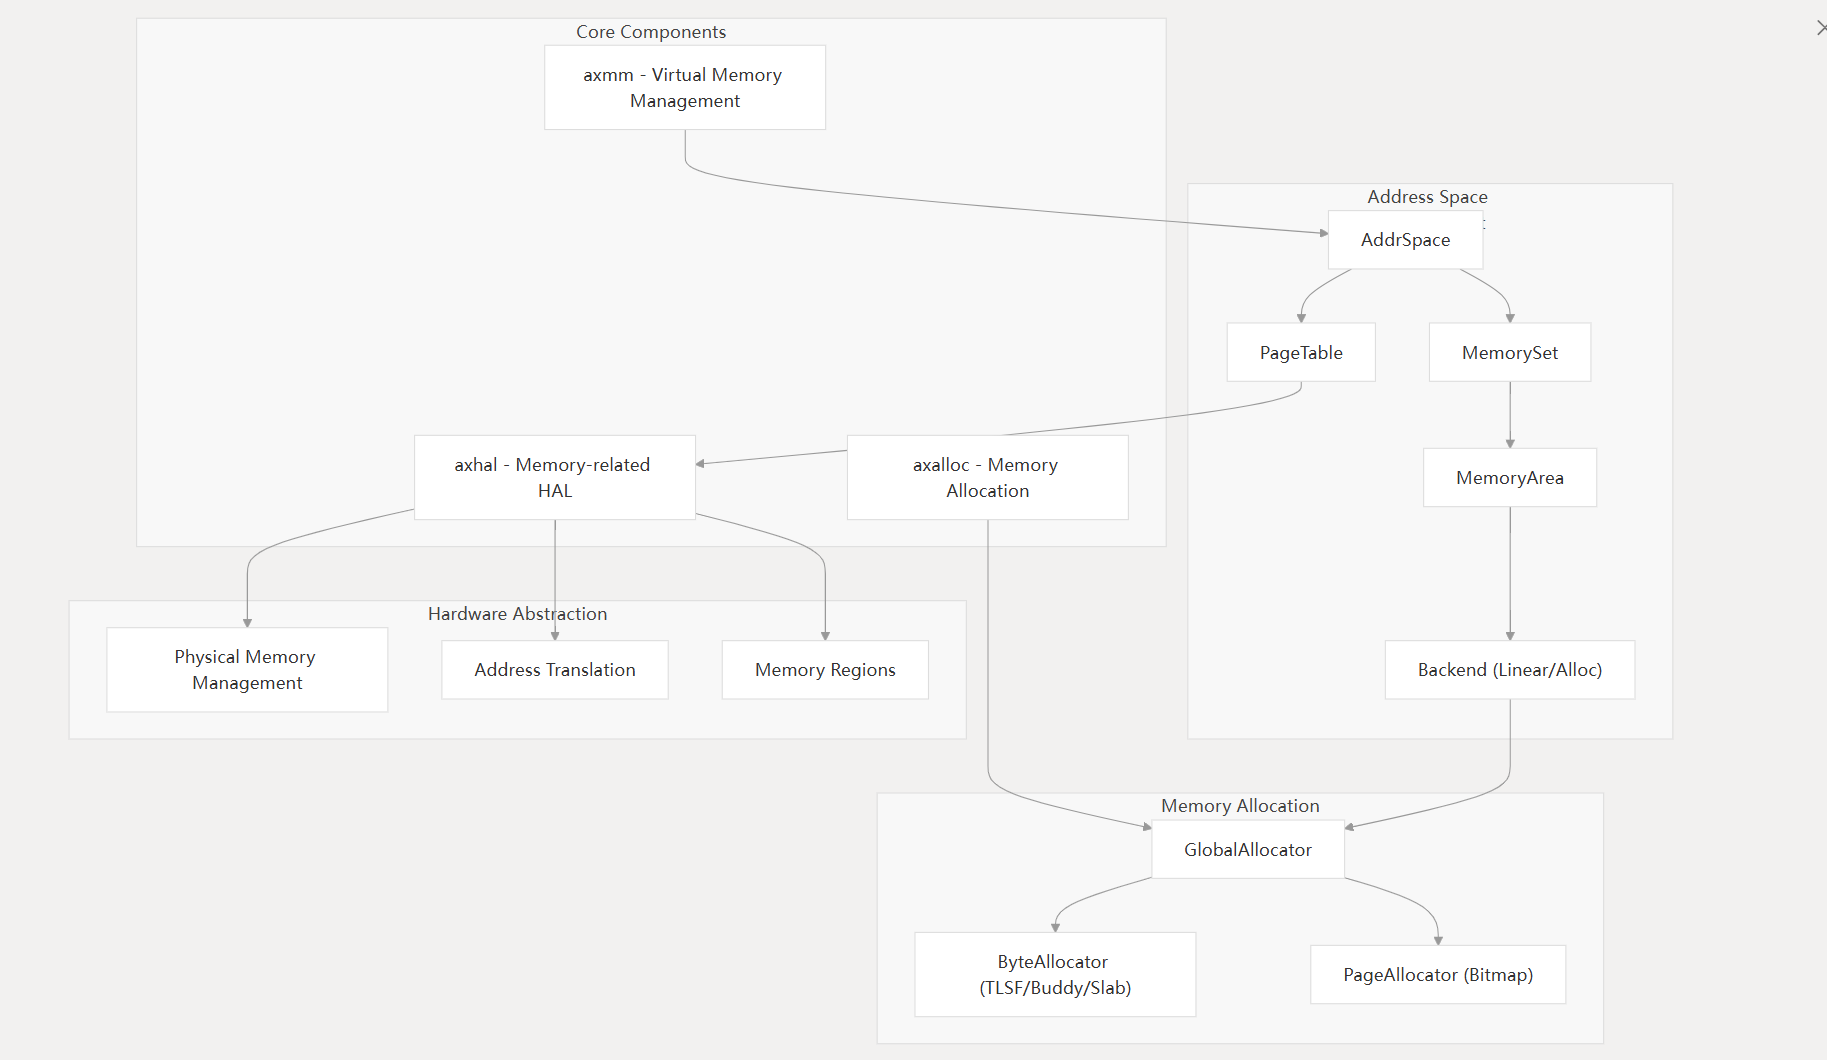
\includegraphics[width=1\linewidth]{arch.png}
  \caption{ArceOS 内存管理系统}
  \label{fig:ArceOS-mm}
\end{figure}

\subsection{axhal}

axhal 组件提供了一层针对不同硬件平台的硬件封装,它为指定的操作平台进行引导和初始化过程,并提供对硬件的操作。在内存方面,axhal 同样进行了一系列的封装操作来支持内存管理。例如:

\begin{itemize}
\item 页表管理封装:axhal 模块将不同架构的页表统一封装为 PageTable 类型,并提供了一致的操作接口,
例如 alloc\_frame(通过页表分配物理页帧)、dealloc\_frame(通过页表释放物理页帧)、phys\_to\_virt(将物理地址转换为虚拟地址)、set\_kernel\_page\_table\_root(设置内核页表根地址)和kernel\_page\_table\_root(获取内核页表根地址)等。
\item 内存区域封装:axhal 模块中定义了 MemRegion 结构体,用于表示和架构无关物理内存区域。MemRegion 结构体包含起始物理地址、区域大小、区域标志和区域名称等属性。通过该结构体,可以方便地管理和操作物理内存区域。
\item 获取内存区域的函数封装:axhal 提供 kernel\_image\_regions、default\_mmio\_regions、default\_free\_regions 接口用于获取内核映像区域、默认 MMIO 区域和默认空闲区域的内存区域列表,并将其封装为 MemRegion 类型。默认的 MMIO 区域和默认空闲区域的位置由 axconfig 模块定义,在不同的硬件平台上可能会有所不同。
\end{itemize}

\begin{figure}
  \centering
  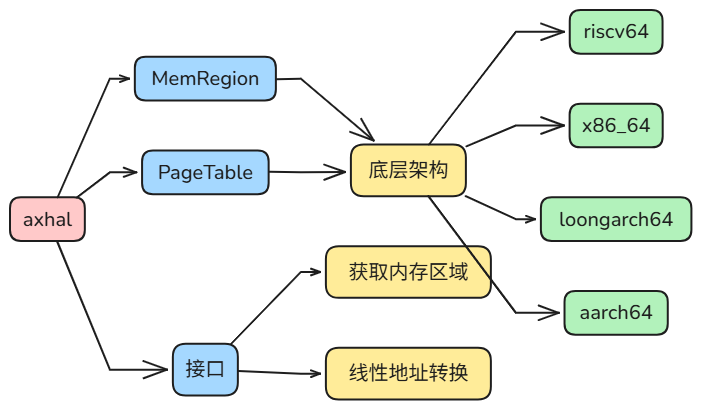
\includegraphics[width=1\linewidth]{axhal-arch.png}
  \caption{axhal 内存管理相关结构图}
  \label{fig:axhal-arch}
\end{figure}



\subsection{axalloc}

\begin{figure}
  \centering
  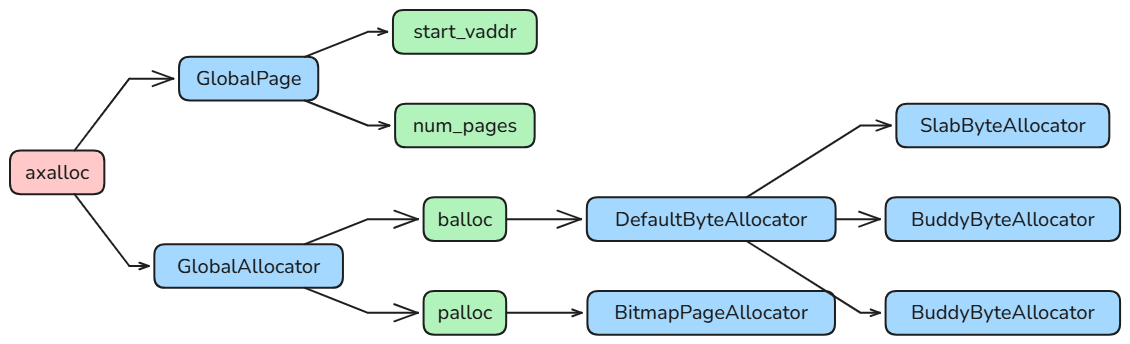
\includegraphics[width=1\linewidth]{axalloc-arch.png}
  \caption{axalloc 结构图}
  \label{fig:axalloc-arch}
\end{figure}

如图\ref{fig:axalloc-arch},axalloc 模块中定义了全局内存分配器 GlobalAllocator,由字节分配器和页面分配器组成。其中,字节分配器用于小内存块的分配和释放,在 ArceOS 中我们提供了三种不同的字节分配器:
\begin{itemize}
\item SlabByteAllocator——基于 slab 分配算法的字节分配器,其核心思想是将内存按照对象的大小进行分类,对于每一类对象,预先分配好一组连续的内存块,这些内存块组成一个 “slab”。每个 slab 包含了多个相同大小的对象槽(Object Slots),当需要分配某个特定大小的对象时,就从对应的 slab 中获取一个空闲的对象槽;当对象释放时,对应的对象槽又可以被重新利用。同时,为了更好地管理这些 slab,会有 slab 缓存(Slab Cache)机制,用于跟踪空闲和已使用的 slab 等状态。
slab 算法对于频繁分配和释放相同类型、相同大小对象的场景表现卓越,同类型对象集中存放使得在数据访问时对 CPU 缓存的利用更为充分,并且可以有效地减少内存碎片。但固定大小的 slab 可能会导致内存浪费和对于多样化、大小不一的内存分配需求适应性较差的问题。
\begin{figure}
  \centering
  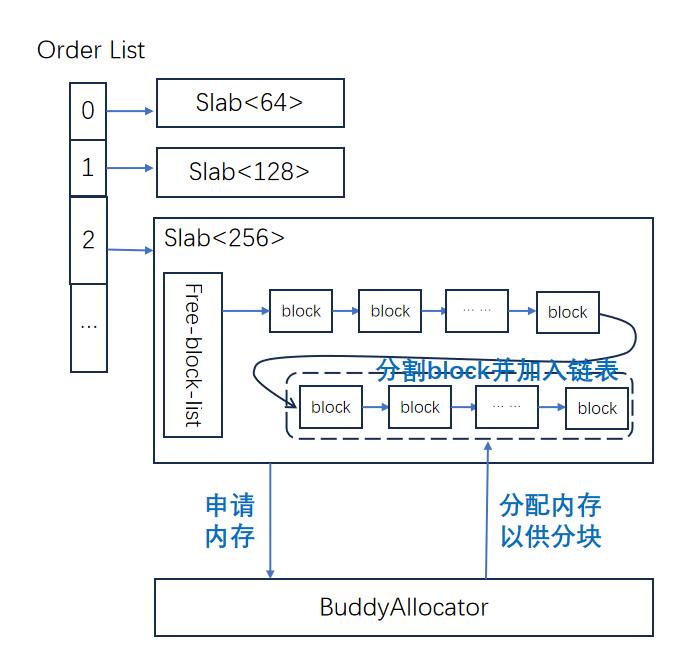
\includegraphics[width=0.7\linewidth]{Slab.png}
  \caption{Slab 算法示意图}
  \label{fig:Slab}
\end{figure}
\item BuddyByteAllocator——基于 Buddy 算法的字节分配器,以一种二叉树的思想来管理内存,它将整个内存空间看作是一个完整的、大小为 2 的幂次方的内存块,当需要分配内存时,如果有符合要求大小(同样是 2 的幂次方)的空闲内存块,就直接分配;若没有,则将更大的空闲内存块不断地二等分(即找到它的 “buddy”,也就是相邻且同样大小的另一半内存块),直到得到合适大小的内存块进行分配。在内存释放时,会检查释放的内存块与其 buddy 是否都空闲,如果是,则将它们合并成一个更大的空闲内存块,如此不断向上合并,直到不能合并为止。
Buddy 算法通过不断地合并空闲的 “伙伴” 内存块,能让内存空间保持相对规整,避免出现大量零散的小空闲块,内存释放时的合并操作判断和执行合并的过程也相对简单高效,但内存分配粒度受限于 2 的幂次方,可能会导致内存浪费和内部碎片问题。
\begin{figure}[H]
  \centering
  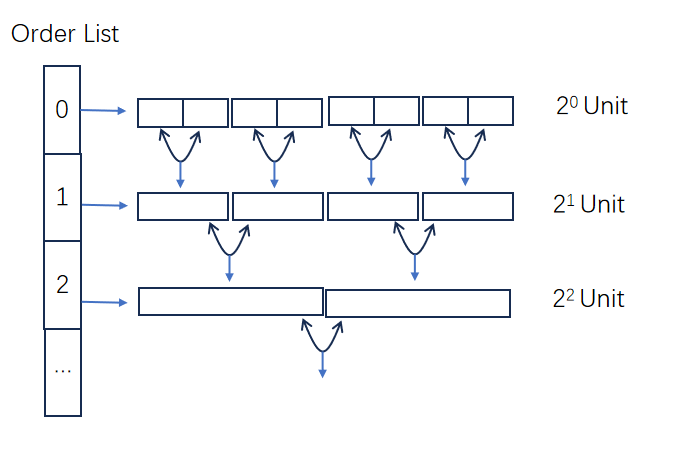
\includegraphics[width=0.7\linewidth,]{Buddy.png}
  \caption{Buddy 算法示意图}
  \label{fig:Buddy}
\end{figure}
\item TlsfByteAllocator——基于 TLSF(Two-Level Segregate Fit)算法的字节分配器,TLSF 采用了两级的分离适配结构。第一级是将整个内存空间按照不同大小范围划分成多个区间,每个区间对应着不同大小的内存块类别,形成一个区间链表。第二级则是针对每个区间,再使用一个位图(Bitmap)和一个空闲块链表来管理该区间内具体的空闲内存块。在进行内存分配时,先根据要分配的内存大小确定所属的区间,然后在位图中查找是否有合适的空闲块,若有则从对应的空闲块链表中取出进行分配;内存释放时,将释放的内存块重新插入到对应的空闲块链表,并相应更新位图信息。
TLSF 算法具有高效的分配速度和高内存利用率,可以灵活应对各种不同大小内存块的分配情况,但是维护两级结构中的各种管理信息使得内存开销相对较大。
\begin{figure}[H]
  \centering
  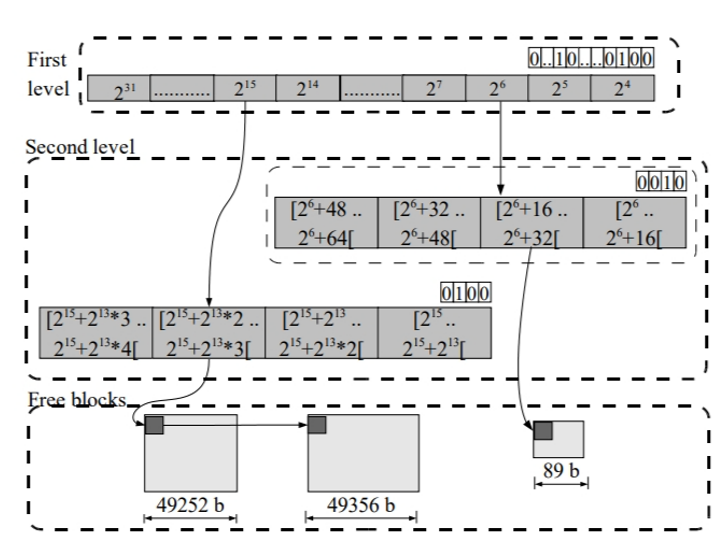
\includegraphics[width=0.7\linewidth]{TLSF.png}
  \caption{TLSF 算法示意图}
  \label{fig:TLSF}
\end{figure}
\end{itemize}

页分配器负责大型分配和扩展字节分配器,使用了标准库中的 BitmapPageAllocator,它是一个基于位图(bitmap)的页粒度内存分配器。它通过使用位图中的每一位来表示一个内存页的分配状态,从而实现高效的内存管理。该分配器支持不同大小的内存分配(从256MB到1TB),并且可以处理不同页大小(PAGE\_SIZE)的情况,要求页大小必须是2的幂次方。它提供了初始化内存区域、分配和释放内存页等基本功能,同时支持对齐分配和指定地址分配等特性。

全局内存分配器通过接口函数提供了对物理内存的操作功能,包括内存的分配、释放、查询等。其主要功能如下:
\begin{itemize}
\item 内存分配器类型选择:通过 Cargo 特性,axalloc 支持用户可以根据需求在 Buddy 分配器、Slab 分配器、TLSF 分配器中选择一种作为全局内存分配器的字节分配器部分。
\item 全局内存分配器初始化:axalloc 定义了一个静态全局变量 GLOBAL\_ALLOCATOR,
并实现了 core::alloc::GlobalAlloc 特性,将其注册为标准库的默认分配器。
在初始化时,需要调用global\_init函数,该函数会初始化页分配器和字节分配器。
\item 内存分配与释放:包括字节分配和释放、页面的分配和释放。
\item 内存状态查询:axalloc 提供了一些函数用于查询内存分配器的状态,如当前内存使用量、空闲内存量等。
\end{itemize}

另外,axalloc 模块提供了用于管理全局内存页面的类型 GlobalPage,其属性包括起始地址和包含的页数。并在全局内存分配器的支持下,提供分配单页和连续页面、填充页面等接口。同时,通过实现 Drop 特性,确保在 GlobalPage 被销毁时,自动释放其占用的内存。这种机制确保了内存资源的高效利用,避免了内存泄漏。

\subsection{axmm}

使用 axalloc 模块提供的内存管理功能,我们已经可以构建起一个简单的内存管理系统,支持内核和应用程序都处于同一地址空间,并且相互可见。
但是,在多任务或多进程的环境下,内核和应用程序之间的内存隔离是非常重要的。为了实现这一点,ArceOS 引入了 axmm 模块来实现虚拟内存管理,其结构如图所示。

\begin{figure}
  \centering
  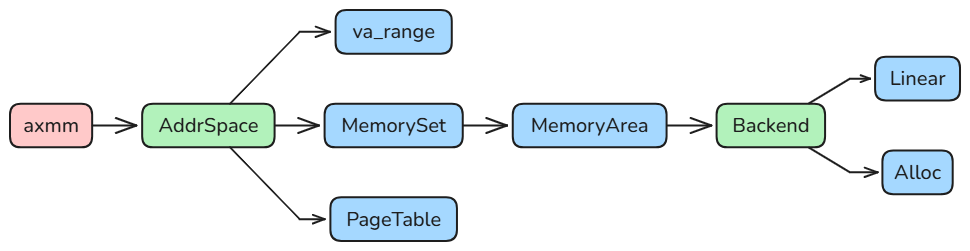
\includegraphics[width=1\linewidth]{axmm-arch.png}
  \caption{axmm 结构图}
  \label{fig:axmm-arch}
\end{figure}


axmm 模块的核心是 AddrSpace 结构体,它表示一个虚拟内存地址空间,包含虚拟地址范围、内存区域集合以及页表。通过该结构体提供的接口,可以对虚拟内存地址空间进行管理,包括创建、映射、解除映射、读写数据等操作。
AddrSpace 的具体接口如图\ref{fig:AddrSpace}所示:
\begin{figure}
    \centering
    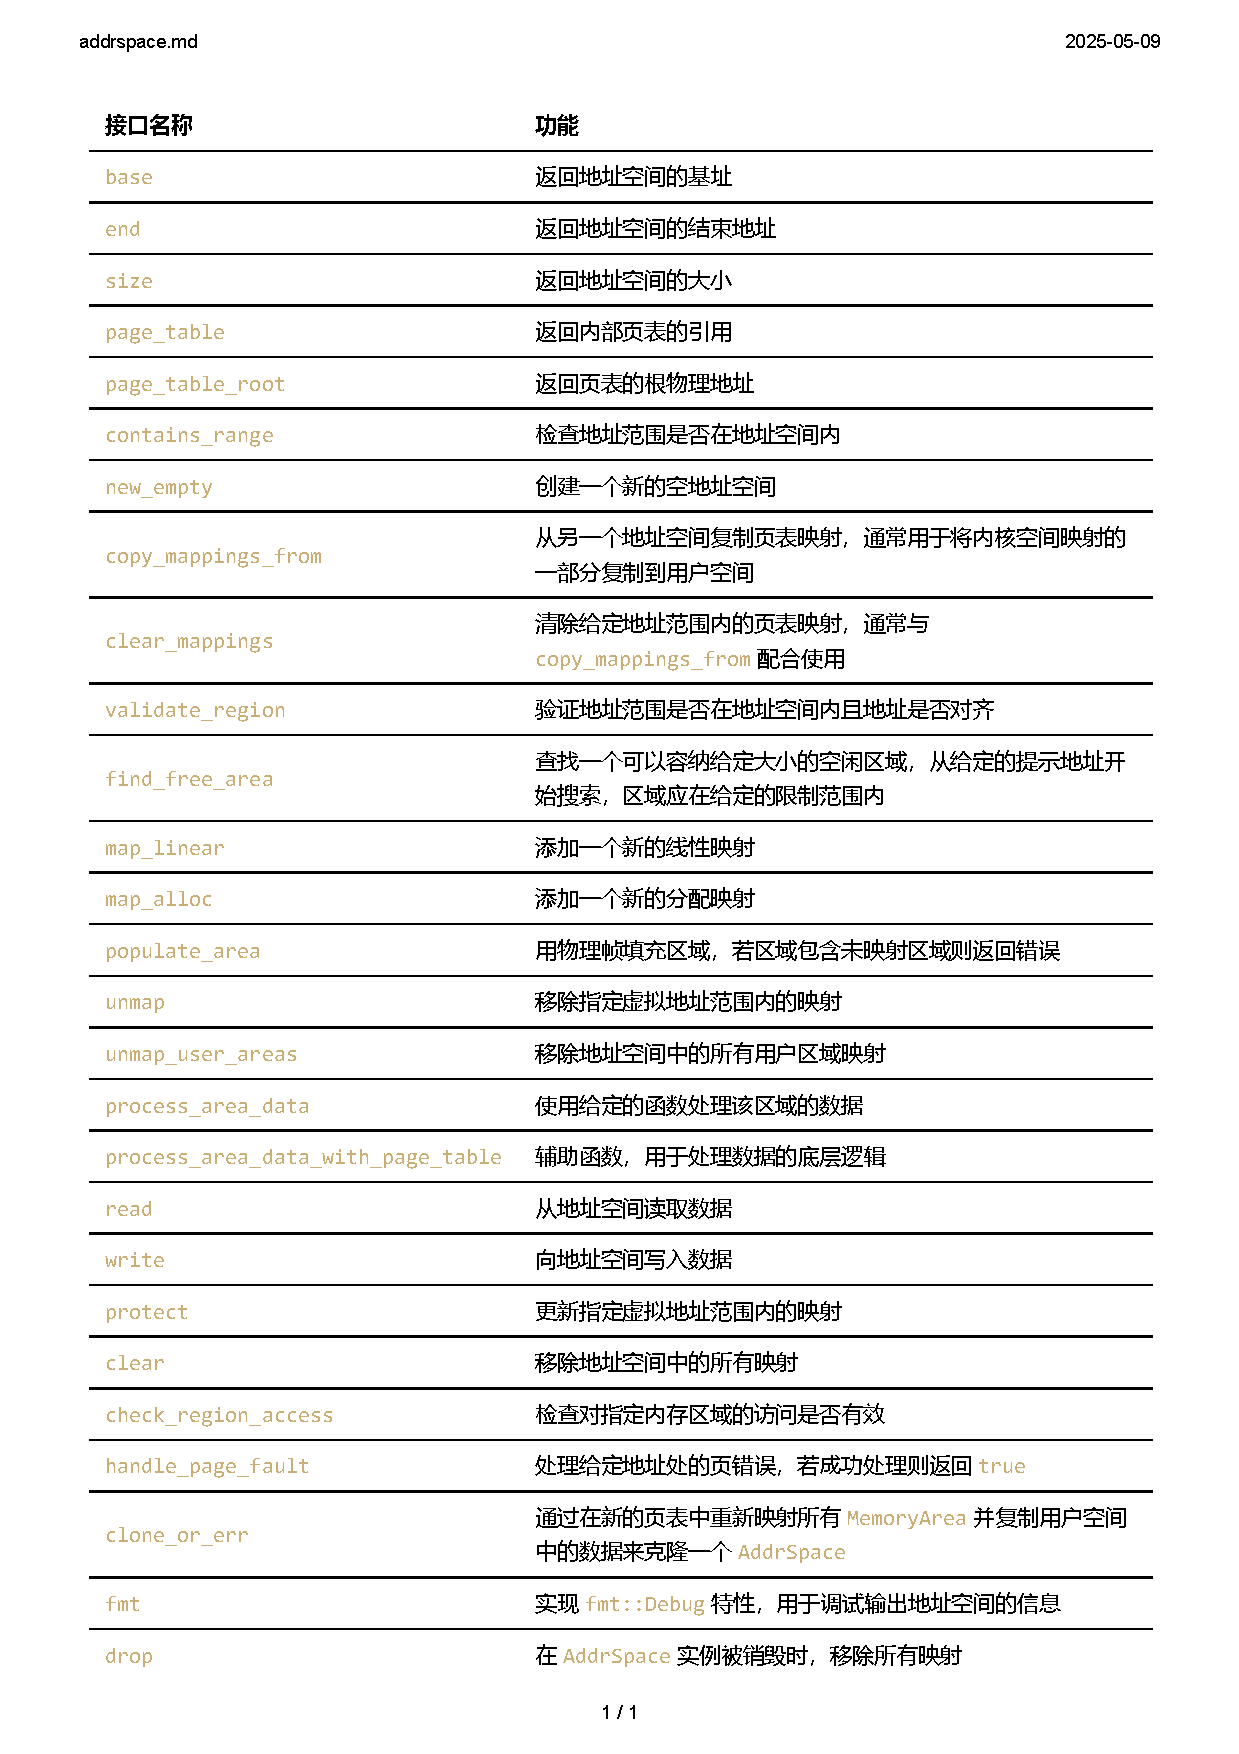
\includegraphics[width=1\linewidth]{addrspace.pdf}
    \caption{AddrSpace 结构体接口}
    \label{fig:AddrSpace}
\end{figure}

实现 AddrSpace 结构体及其接口对于构建一个高效、灵活且安全的虚拟内存管理系统具有极其重要的意义。一方面,通过为每个进程分配独立的虚拟地址空间,AddrSpace 不仅实现了内核与用户空间的隔离,还确保了进程之间的相互独立,从而防止了进程间的非法访问和潜在的破坏行为。

另一方面,AddrSpace 提供的内存保护机制进一步增强了系统的安全性。它通过页表和访问权限控制,确保每个进程只能访问自己被授权的内存区域,同时在检测到非法访问时能够及时触发异常并进行处理,从而避免系统崩溃。这种机制不仅保护了内核的稳定性,还为用户程序提供了可靠的运行环境。

除 AddrSpace 结构体及其接口外,axmm 模块还定义 Backend 核心抽象,用于处理不同类型的内存映射实现细节。它作为 MemoryArea (内存区域)的后端,将虚拟地址与物理存储关联起来,将映射、解除映射、处理页面异常等操作传递到具体的后端实现,进而完成对页表的操作。axmm 模块支持两种类型的内存映射后端:
\begin{itemize}
\item Linear Backend:用于与已知物理地址的直接映射,例如内存映射的 I/O 区域或内核映像部分,虚拟地址和物理地址具有固定的偏移关系;
\item Allocation Backend:按需分配物理页,支持延迟分配,常用于用户空间内存管理。
\end{itemize}

内存区域对应的映射类型在内存区域对象创建时,即调用 AddrSpace 的 map\_linear 或 map\_alloc 方法申请空间并进行映射时指定。

\subsection{axdma}
axdma 模块实现了 DMA 内存管理,提供了直接内存访问的接口。DMA(Direct Memory Access,直接内存访问) 是一种硬件特性,允许某些硬件子系统在不经过 CPU 控制的情况下直接访问系统内存,
DMA 通常用于高速数据传输,例如从硬盘读取数据到内存,或者从内存将数据发送到网络接口。

在传统的数据传输中,CPU 需要逐字节地从外设读取数据,然后将其写入内存,或者从内存读取数据后写入外设。这种操作不仅效率低下,还会占用大量的 CPU 时间。而 DMA 允许外设直接访问内存,
无需 CPU 参与,从而提高了数据传输的速度和效率,并释放了 CPU 的计算资源,使其可以处理其他任务。

\begin{figure}[H]
    \centering
    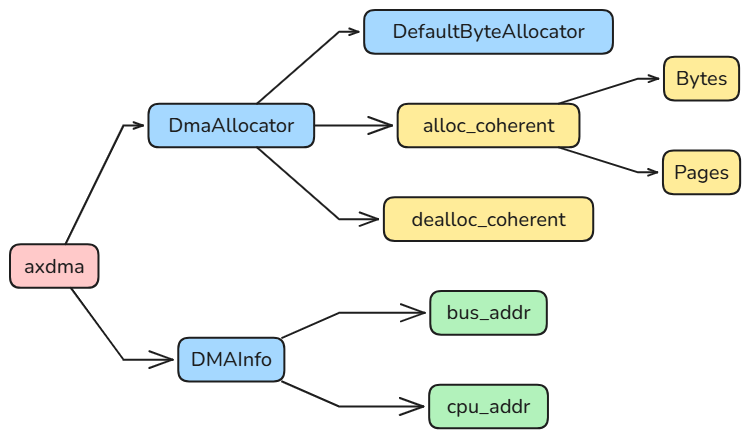
\includegraphics[width=1\linewidth]{axdma-arch.png}
    \caption{axdma 结构图}
    \label{fig:axdma-arch}
\end{figure}

如图\ref{fig:axdma-arch},ArceOS 的 DMA 模块通过实现 DMA 分配器(DmaAllocator),向设备驱动模块(axdriver)提供了 DMA 内存分配和释放的接口。
它会根据设备的需求,分配合适大小的内存块,并在 DMA 操作完成后释放这些内存块。
DMA 分配器还会处理 DMA 操作中的地址转换问题,将虚拟地址转换为总线地址,以便于 CPU 访问。
DMAInfo 结构体则记录了用于 DMA 操作的内存区域相关的信息,包括 CPU 访问该区域的虚拟地址和该区域在总线上的物理地址。
同时,DMA 分配器分配的内存需要标记为 UNCACHED,以避免缓存一致性问题,这需要虚拟内存管理模块(axmm)提供的接口来完成。

DMA 模块的具体接口如图\ref{fig:DmaAllocator}所示:
\begin{figure}[H]
    \centering
    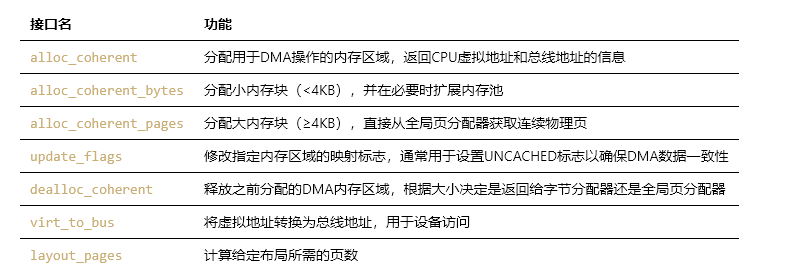
\includegraphics[width=0.7\linewidth]{axdma.png}
    \caption{DmaAllocator 结构体接口}
    \label{fig:DmaAllocator}
\end{figure}

\section{ArceOS 内存管理机制}

% ArceOS 中与内存管理相关的结构主要有:

% \begin{itemize}
% \item MemRegion:表示一个物理内存区域,包含起始物理地址、区域大小、区域标志和区域名称。
% \item GlobalAllocator:全局内存分配器,用于管理物理内存区域,包含用于小分配的字节分配器和用于大型分配和扩展字节分配器的页分配器,提供了内存和页面的分配和释放接口。
% \item AddrSpace:表示虚拟内存地址空间,包含虚拟地址范围、内存区域集合以及页表。通过该结构体提供的接口,可以对虚拟内存地址空间进行管理,包括创建、映射、解除映射、读写数据等操作。
% \item MemoryArea:表示一块虚拟内存区域,包含起始地址、结束地址、访问权限和映射关系等信息。
% \item MemorySet:表示虚拟内存区域的集合构成的 Btree 结构,提供管理虚拟内存区域的具体方法。
% \item Backend:内存映射后端,包括 Linear Backend 和 Allocation Backend。
% \end{itemize}

在本章第一节中我们提到了 ArceOS 的启动和初始化过程,而在这里我们将对其中与内存分页相关的部分进行详细分析:
架构的初始化函数 \_start 中进行了启动页表和内存管理单元的初始化,为 QEMU 虚拟机的物理内存等关键区域构建映射,设置根页表地址并刷新 TLB,完成分页的早期启动阶段。
这一阶段是 ArceOS 默认开启的,构建的映射为恒等映射,虚拟地址和物理地址相同,主要用于内核的启动和初始化。
\begin{lstlisting}[language=c, caption=\_start]
phys_virt_offset = const PHYS_VIRT_OFFSET,
boot_stack_size = const TASK_STACK_SIZE,
boot_stack = sym BOOT_STACK,
init_boot_page_table = sym init_boot_page_table,
init_mmu = sym init_mmu,
\end{lstlisting}

如图~\ref{fig:init}所示,分页的早期启动阶段完成后,如果开启了 paging 特性,在 rust\_main 函数中会调用 axmm 模块的 init\_memory\_management 函数初始化内存管理,
即创建内核的虚拟地址空间,为内核的虚拟地址空间构建线性映射,调用 axhal 的接口设置内核的虚拟地址空间的页表,并将其设置为当前的页表根,完成分页的重建映射阶段。
该阶段将内核和用户空间的虚拟地址空间隔离开来,让内存管理模块能够管理更大的地址空间,为 DMA 和多任务等功能提供支持。

\begin{figure}[H]
    \centering
    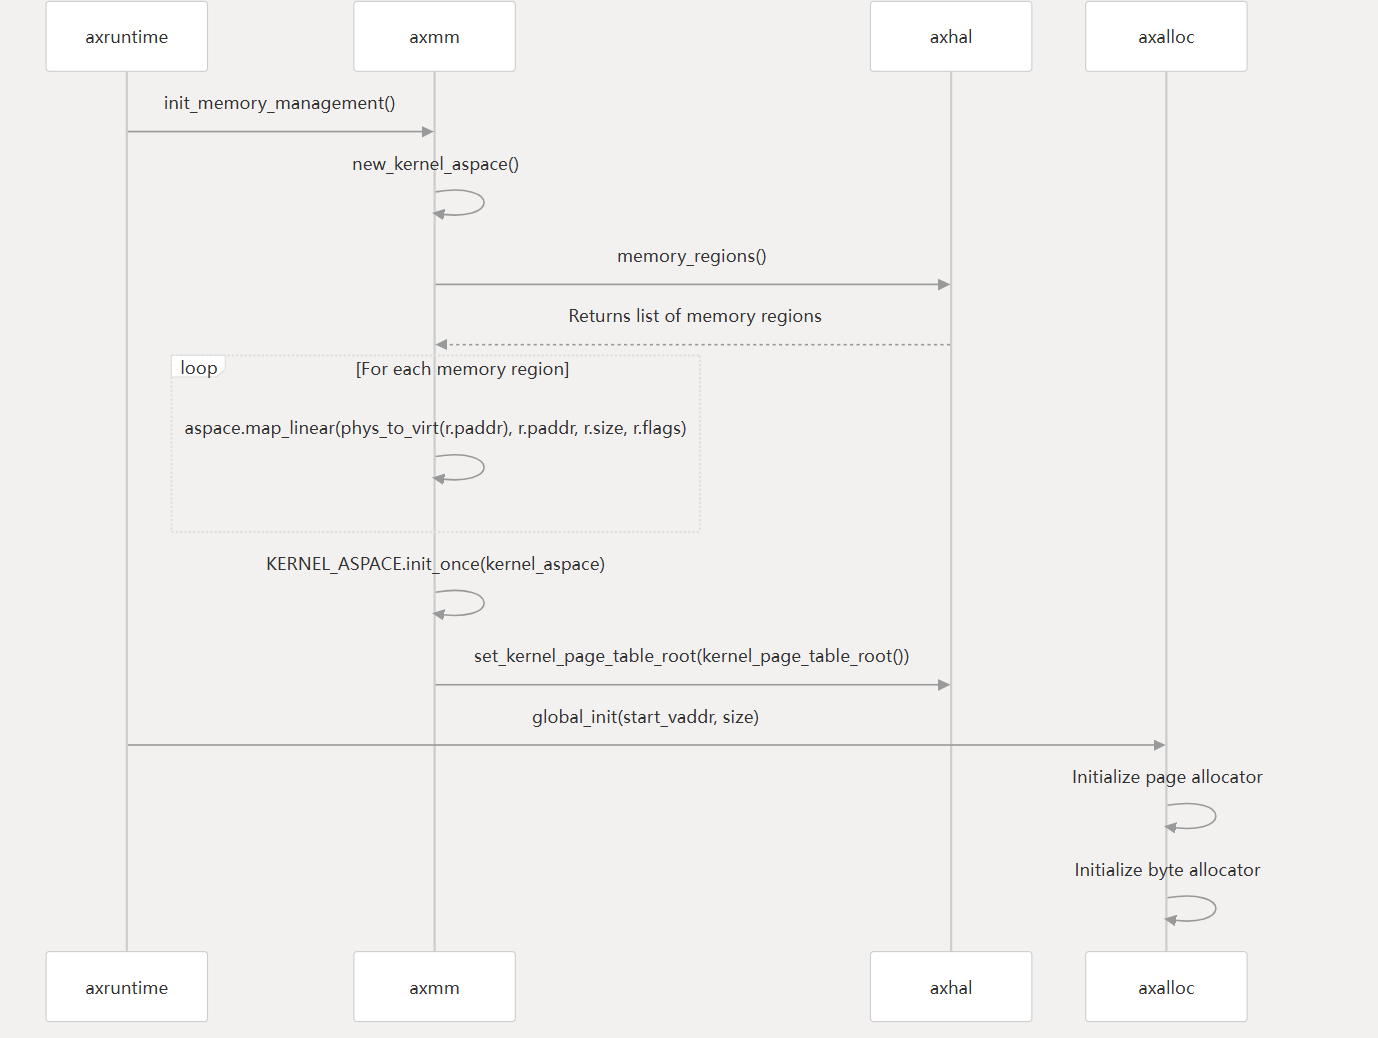
\includegraphics[width=1\linewidth]{init.png}
    \caption{分页的重建映射阶段}
    \label{fig:init}
\end{figure}

开启 paging 特性且上层架构或者应用需要对内存空间进行操作时,会调用 AddrSpace 的相应接口,如 find\_free\_area(寻找空闲内存区域)、map\_linear(建立线性映射)、map\_page(建立分配映射)等方法,这些方法会根据具体的内存操作需求,对页表和虚拟地址空间进行操作,并调用全局内存分配器进行物理内存的分配和释放。全局分配器在分配时会先尝试从字节分配器分配,如果字节分配器内存不足,则计算需要多少内存,从页面分配器分配页面后将页面添加到字节分配器重新进行分配,此方法允许高效处理小型和大型分配,同时保持合理的内存使用率。

同时,ArceOS 还在 AddrSpace 结构体中提供了页面异常的处理接口,例如当访问的虚拟地址对应的物理页不存在时,会触发缺页异常,此时会调用 AddrSpace 的 handle\_page\_fault 函数处理缺页异常,
该函数会对后端为 Alloc 类型的地址,调用 axalloc 中的全局内存分配器进行物理页的分配,并通知 axhal 中的页表更新映射关系。对于后端为 Linear 类型或者需要填充的地址,则会处理失败,返回 false,
因为这两类的地址在创建时就应完成物理页的分配和映射,缺页异常的处理不适用。AddrSpace 的 handle\_page\_fault 函数的流程图如图~\ref{fig:handle-page-fault-arceos}所示:

\begin{figure}[H]
    \centering
    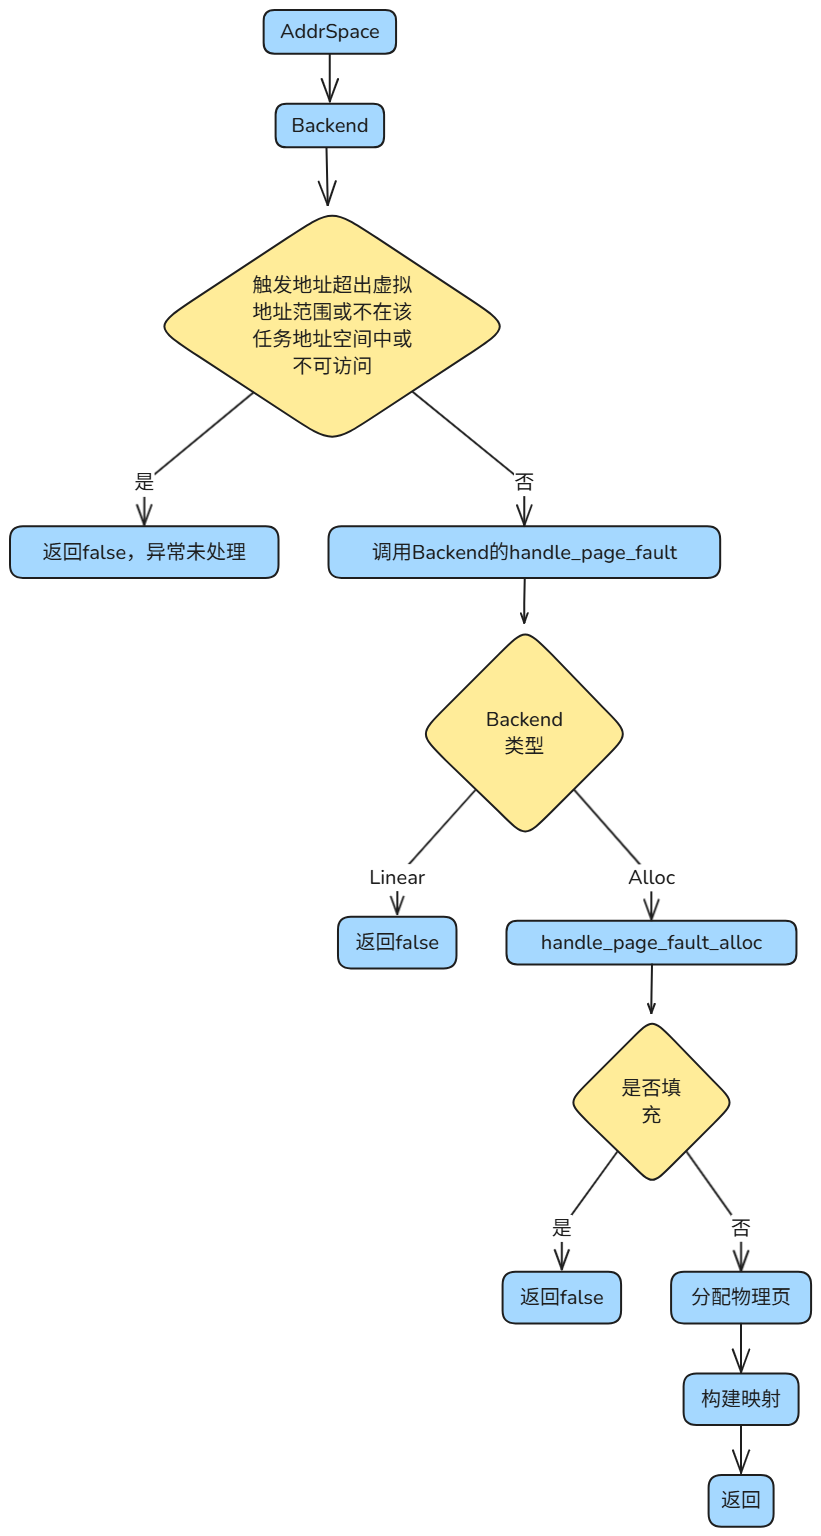
\includegraphics[width=0.7\linewidth]{pagefault-arceos.png}
    \caption{handle\_page\_fault 函数流程图}
    \label{fig:handle-page-fault-arceos}
\end{figure}


借助缺页异常的处理,ArceOS 还实现了 Lazy Map 机制,即当访问的虚拟地址对应的物理页不存在时,不会立即分配物理页,而是在第一次访问该虚拟地址时才触发缺页异常,进行分配和映射。